%************************************************
\chapter{Introduction}
\label{chapter:introduction}
%************************************************

An intelligent system thinks about a problem domain, learning the
effects of its actions, constructing and executing plans to accomplish
its goals.  I will refer to these types of thinking about a problem
domain as deliberative thinking.  A reflective intelligence extends
the deliberative intelligence by learning to accomplish goals in its
own deliberative thinking process.  Reflective thinking is sometimes
referred to as ``thinking about thinking'' or ``metacognition.''  A
reflective intelligence can learn to select between different types of
thinking that are appropriate for generating plans toward different
types of goals.  In this thesis, I present the Substrate for
Accountable Layered Systems (SALS), an open-source
\begin{wrapfigure}{r}{6.125cm}
  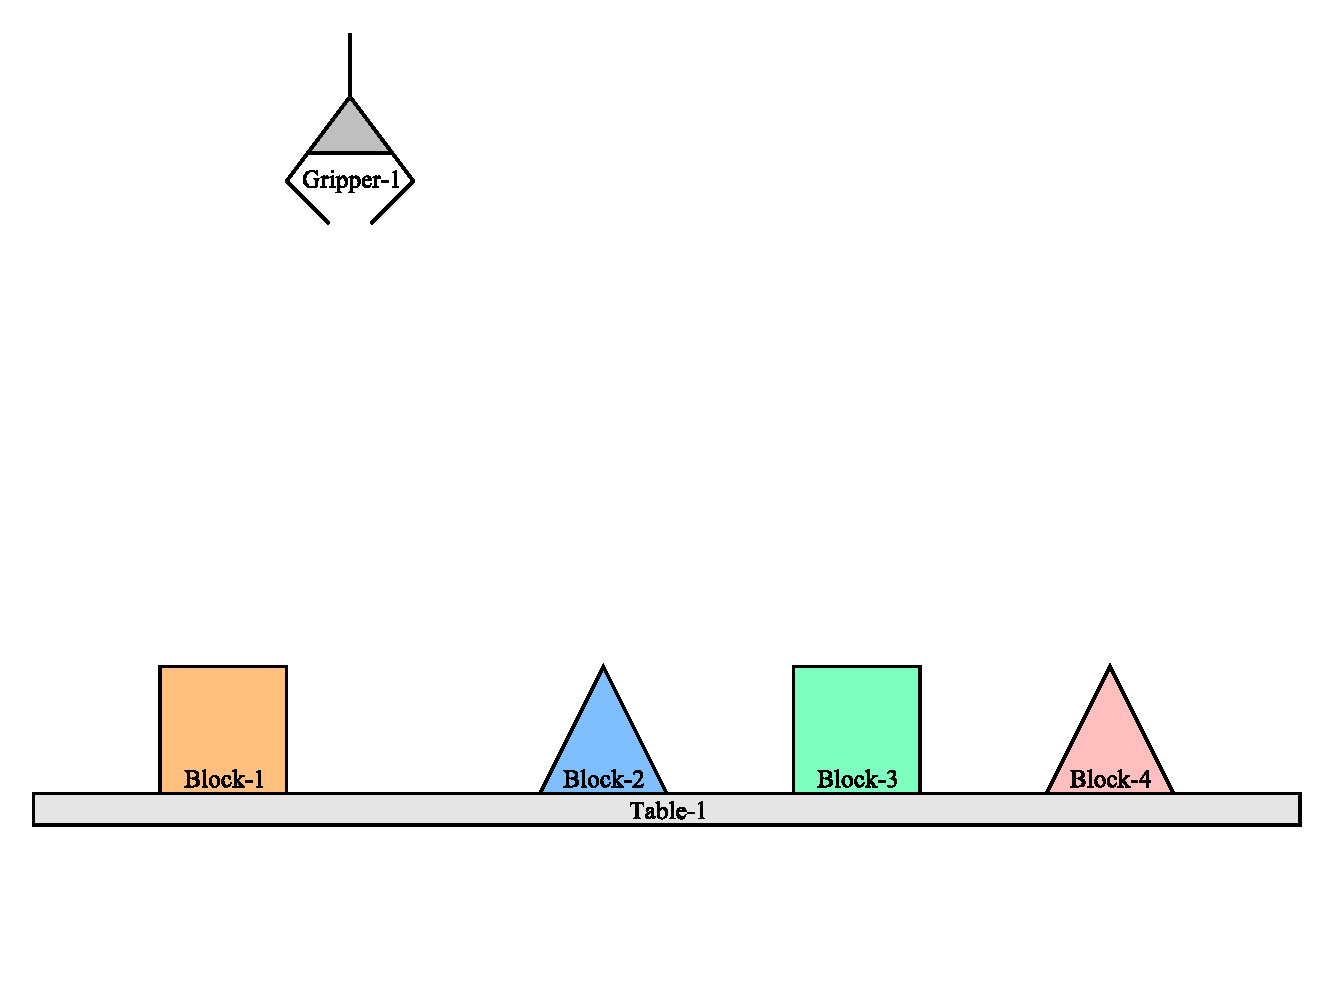
\includegraphics[width=6cm]{gfx/blocks_world_large-01}
  \caption[An example ``Blocks World'' problem domain.]{An example
    ``Blocks World'' problem domain.}
  \label{figure:introduction_example_problem_domain}
\end{wrapfigure}
software platform for the development of experimental reflective
Artificial Intelligences (AI).  A deliberative AI system consists of
three processes: {\mbox{(1)~perceptual}} data are generalized and
categorized to learn abstract models, {\mbox{(2)~abstract}} models are
used to infer hypothetical states, i.e. states of future, past, or
otherwise ``hidden'' variables, {\mbox{(3)~actions}} are chosen based
on considerations of hypothesis dependent inferences.  There are many
approaches to machine learning that focus on this abstract 3-step
closed-loop process of learning to control: reinforcement learning
\cite[]{kaelbling:1996,dvzeroski:2001}, game theory
\cite[]{bowling:2000,rapoport:2001}, and control theory
\cite[]{simon:1982, bertsekas:1995}.  The discipline of computational
metacognition \cite[]{cox_and_raja:2008,cox:2010} focuses on making at
least two layers of closed-loop systems.  Organizing the three-step
architecture within the metacognitive framework, deliberative thinking
is modeled as a closed-loop learning algorithm that perceives and
learns to control the external world, while reflective thinking is
modeled as a second closed-loop learning algorithm that perceives and
learns to control the deliberative thinking process.  While it may be
clear how to trace the inputs to deliberative thinking, there is not a
consensus in the literature on a tractable approach to modeling the
inputs to reflective thinking.  In this thesis, I present a tractable
approach to reflective thinking that scales to $N$ layers of
reflective control.

\section{Contributions}

The four contributions of this thesis are:
\begin{enumerate}
\item \emph{Emotion Machine Cognitive Architecture}: A computational
  implementation of the bottom four layers of the ``Emotion Machine''
  six-layered theory of mind \cite[]{minsky:2006}.  The implementation
  contains a physical simulation that is controlled by a deliberative
  physical object-level reasoning layer with another reflective
  meta-level reasoning layer that learns to control the deliberative
  problem solving resources.  The architectural primitives include
  resources that are organized into agencies that are organized into
  layers.  The implementation includes five layers that are described
  in
  {\mbox{\autoref{chapter:emotion_machine_cognitive_architecture}}}:
  (1) built-in reactive thinking, (2) learned reacting thinking, (3)
  deliberative thinking, (4) reflective thinking, and (5)
  super-reflective thinking.  The implementation leaves
  self-reflective and self-conscious layers of the Emotion Machine
  theory as future extensions of this research.
\item \emph{Learning from Being Told Natural Language Plans}: A system
  needs a plan library.  Plan libraries can be authored by humans as
  sequences of simple natural language sentences.  The implementation
  includes the ability to interpret and imagine executing natural
  language commands by using analogies to natural language plans that
  it already knows.  In this case, ``being told'' means that a natural
  language plan is programmed into the AI by the user.  Interpreting a
  natural language plan involves parsing the English and generating a
  compiled program, along with imagined hypotheses about the program's
  effects.  These guesses are based on what partial states the plan
  checks for in the control domain as well as rules learned from
  previous executions of similar actions in the past.
\item \emph{Learning Asynchronously from Experience}: Executing plans
  in the external problem domain gives the system better expectations
  for what plans will actually end up doing when they are interpreted
  ({\mbox{\autoref{section:natural_language_plans_interpreting_natural_language_plans}}}),
  imagined
  ({\mbox{\autoref{section:imagining_the_effects_of_ambiguous_natural_language_plans}}})
  and executed
  ({\mbox{\autoref{section:two_experiential_event_streams_flow_to_each_planning_layer}}}).
  I refer to this form of learning the effects of actions in the
  problem domain as learning from ``experience.''  Many types of
  failures can occur when interpreting, imagining and actually
  executing ambiguous natural language plans.  These experiences of
  different types of failures inform reflective learning algorithms to
  subsequently predict these types of plan failures.  Learning from
  experience is executed concurrently and asynchronously with the
  currently executing plan.  The learning algorithm receives a stream
  of frame mutation trace events from the currently executing plan and
  uses this stream to learn abstract causal rule-based models.  In
  this way, effects of physical and mental actions are learned through
  experience without slowing down the primary plan execution speed.
  Such failures are input to the reflective layer, which can learn to
  predict and avoid these failures in the future.
\item \emph{Virtual Machine and Programming Language}: A concurrent
  and parallel virtual machine and low-level Lisp-like programming
  language provide the foundation upon which all of the above
  contributions have been implemented.  The virtual machine includes
  native procedural tracing features that facilitate the automatic
  monitoring and control of many concurrently executing tasks.  The
  virtual machine takes advantage of multiple CPU and multiple-core
  CPU hardware configurations.  The programming language is a bytecode
  compiled language and all code for all contributions are open
  source.
\end{enumerate}

\section{A Story of Reflective Learning}

Before getting into abstract generalizations of reflective thinking,
let us consider the advice of Seymour Papert: ``You can't think about
thinking without thinking about thinking about something.''  Following
this advice, consider the simple physical block stacking world,
depicted in {\autoref{figure:introduction_example_problem_domain}},
which is similar to the ``Blocks World'' planning domain
{\cite[]{winograd:1970}}.  Imagine that the robot arm in this simple
scenario is an entirely deliberative (non-reflective) AI that wants to
accomplish the deliberative goal of a block being on a block.  This AI
has the capability of learning both from experience as well as from
being told knowledge.  The deliberative AI has been told a number of
natural language plans for how to pick up and move around blocks in
this problem domain.  What types of thoughts might be going through
the mind of this deliberative block stacking AI?  The following story
might be what this type of deliberative AI would be thinking in this
block stacking domain:
\begin{quote}
  I want to accomplish the deliberative goal of a block being on a
  block.  I must choose how to physically act.  I have a number of
  plans that I have been told, but I don't know what they will do.  I
  am focused on my most recently learned plan for how to physically
  act, which is called, ``stack a cube on a pyramid.''  I have been
  told this plan in natural language, so I must interpret what it
  means if I am going to imagine executing it.  If I can imagine a way
  that this plan could accomplish my deliberative goals, I will
  execute it.  I will try interpreting and imagining the physical
  effects of my most recently learned plan for physical action,
  ``stack a cube on a pyramid.''  I imagine that executing this plan
  will accomplish my goal of a block being on a block.  I will stop
  imagining the rest of my plans and try executing this plan for
  physical action.  I am picking up a cube and dropping it on a
  pyramid.  The cube is falling off of the pyramid and onto the table.
  Oh no!  A block is not on a block.  My expectations have failed!  A
  deliberative plan has failed.  I will relearn the physical effects
  of my physical actions based on this new physical knowledge.  The
  next time that I am dropping a block on a pyramid, I will expect the
  block to fall onto the table.  Now, I must stop executing this plan
  and again choose how to physically act, given my new information.
\end{quote}
In this story, the deliberative AI interprets and imagines executing
plans based on reasoning by natural language analogies.  Because the
deliberative AI experiences a knowledge failure, the deliberative AI
learns a better model of the effects of its physical actions.  If this
AI were reflective, it would be able to learn more from the
deliberative failure of the AI in this story.  A reflective AI not
only learns the effects of physical actions but also learns the
effects of deliberative actions, such as the effects of imagining the
effects of a plan.  How would a reflective AI approach thinking about
accomplishing the same physical goal in the same problem domain?  If
the AI were reflective, the following story might be what it would
think to itself as it tries to reflectively decide how to deliberate
about plans for physical action:
\begin{quote}
  I want to accomplish the deliberative goal of a block being on a
  block.  I also want to avoid my negative reflective goal of keeping
  the deliberative layer from having plans that have failed.  I have
  been told a number of reflective plans for deliberative action, but
  I don't know what they will do.  I must choose a reflective plan for
  deliberative action.  I am focused on my most recently learned
  reflective plan, which is called, ``Find and execute a recently
  learned plan to accomplish my goals.''  I choose to imagine the
  effects of the various possible interpretations of this
  underspecified natural language plan on my deliberative knowledge.
  I can adapt other analogous plans to interpret this one, and I
  imagine that at least one interpretation will not lead to any
  deliberative plans having any execution failures, so I choose to
  execute this reflective plan to ``find and execute a recently
  learned plan to accomplish my goals.''
\end{quote}
At this point in the story, the AI has decided on a plan of
deliberative action.  Notice that this story is very similar to the
first story, except rather than deciding on a plan of physical action,
the reflective planner is deciding on a plan for deliberative action.
In this case, the ``find and execute a recently learned plan to
accomplish my goals'' plan is an implementation of a planning
algorithm within the natural planning language itself.  The fact that
the deliberative planning algorithm is written in the reflective
planning language is one key aspect to the recursive nature of this
approach to reflective learning and control.  The reflective AI has a
number of reflective plans for how to deliberatively plan, the method
that the AI chose in this case tries to find a plan that it has been
told most recently.  So, the AI begins executing this reflective plan,
which becomes the deliberative planning process that tries to find a
plan for acting in the physical problem domain:
\begin{quote}
  I will try interpreting and imagining the physical effects of my
  most recently learned plan for physical action, ``stack a cube on a
  pyramid.''  I imagine that executing this plan will accomplish my
  goal of a block being on a block.  I will stop imagining the rest of
  my plans and try executing this plan for physical action.  I am
  picking up a cube and dropping it on a pyramid.  The cube is falling
  off of the pyramid and onto the table.  A block is not on a block.
  Oh no!  My deliberative expectations have failed!  A deliberative
  plan has failed.  Oh no, I was reflectively trying to avoid
  deliberative plan failures!  My reflective expectations have failed!
  A reflective plan has failed.
\end{quote}
At this point in the story, the AI has encountered two failures that
will lead to two opportunities for learning the effects of both its
physical actions as well as its deliberative actions.  If we consider
what the AI might learn from this story, the AI might think:
\begin{quote}
  I have new support for the hypothesis that dropping a block while
  being over a pyramid leads to two blocks being on the table.  I also
  have new support for the hypothesis that executing plans that try to
  accomplish the goal of a cube being on a pyramid may lead to an
  expectation failure when executed.
\end{quote}
The fact that the AI failed at both the deliberative and reflective
levels allowed the AI to learn two new sets of hypotheses: (1) about
physical actions, and (2) about deliberative actions.  The fact that
more can be learned by adding a reflective layer to a learning
algorithm is inspiration for researching reflective machine learning
in those domains where physically acting is relatively costly while
thinking is relatively cheap.  Now, see how the reflective AI
approaches reflectively thinking differently after it has learned from
this initial experience:
\begin{quote}
  I still want to accomplish the deliberative goal of a block being on
  a block.  I still also want to avoid my negative reflective goal by
  keeping the deliberative layer from having plans that have failed.
  I must choose another reflective plan for deliberative action.  I am
  focused on my most recently learned reflective plan, which is
  called, ``Find and execute a recently learned plan to accomplish my
  goals.''  When I imagine executing this plan, I use my learned
  hypothesis that predicts that executing this reflective plan will
  lead to a failure in the deliberative knowledge.  I choose to not
  execute this plan because it does not avoid my negative reflective
  goal.  I focus on my next plan, ``find and execute an old plan to
  accomplish my goals.''  I can adapt other analogous plans to
  interpret this reflective plan, and I have no hypotheses that
  predict that this plan will lead to any deliberative failures, so I
  choose to execute this reflective plan to ``find and execute an old
  plan to accomplish my goals.''
\end{quote}
After this second round of reflective reasoning, the first reflective
plan is considered and again imagined, but this time the reflective
layer predicts that this reflective plan will lead to a failure in the
deliberative layer because the deliberative conditions are so similar.
For example, executing the same reflective plan in the context of the
same deliberative goals is hypothesized to cause a deliberative
failure.  Because this conflicts with the negative reflective goal to
avoid deliberative failures, the first reflective plan is bypassed.
The AI ends up considering another plan and selecting it for
execution.  The difference between these two plans is in how they
organize their search through possible plans.  The first reflective
plan considers deliberative plans that it has learned most recently,
while the second reflective plan considers deliberative plans that it
has learned furthest in the past.  In general, plans may be
reflectively organized in more complicated mental structures, but in
order to simply demonstrate my point, plans are organized in a
doubly-linked list structure that goes forward and backward in time.
One could imagine organizing plans by location, goal, or other equally
important metrics in more complex data structures.  Now that the AI
has reflectively chosen a different way to deliberatively plan, the AI
executes this reflective plan, which becomes the deliberative
reasoning process:
\begin{quote}
  I will try interpreting and imagining the physical effects of my
  oldest plan for physical action, ``stack a pyramid on a cube.''  I
  imagine that executing this plan will accomplish my goal of a block
  being on a block.  I will stop imagining the rest of my plans and
  try executing this plan for physical action.  I am picking up a
  pyramid and dropping it on a cube.  The pyramid is now sitting on
  the cube.  A block is on a block.  Yay!  Executing my oldest plan
  for physical action has accomplished my deliberative goal!  Yay!  I
  have also avoided my negative reflective goal to avoid deliberative
  plan failures!
\end{quote}
So, finally, the reflective AI is happy to accomplish its deliberative
goal.  Note that the deliberative algorithm would have eventually
found and executed the correct deliberative plan, if it had gone
through all of its plans and imagined all of their effects, finally
getting to its oldest plan, which happened to be the successful one.
The advantage of the reflective learning algorithm is that it allows
learning different ways of planning for dealing with different types
of deliberative goals.  Reflective planning allows learning how
different plan representations, planning algorithms, and other
deliberative knowledge is relevant to creating plans toward different
types of deliberative goals.

\section{Layers of Knowledge}

One tricky aspect of programming reflective learning algorithms is
keeping clear distinctions between different layers of knowledge in
the AI.  {\autoref{table:physical_deliberative_reflective_knowledge}}
shows a few examples of physical, deliberative and reflective
knowledge.
\begin{table}
\centering
\begin{tabular}{|p{2cm}|p{8cm}|}
\hline \emph{Physical Knowledge} & \begin{packed_itemize}
\item{A cube is on a pyramid.}
\item{A gripper is moving left.}
\item{A gripper is above a cube.}
\item{A cube is to the left of a pyramid.}
\end{packed_itemize} \\
\hline \emph{Deliberative Knowledge} & \begin{packed_itemize}
\item{Goal 1 is for a cube to be on a pyramid.}
\item{Plan 1 is to stack a pyramid on a cube.}
\item{Plan 1 fails for Goal 1.}
\item{Goal 2 is for a pyramid to be on a cube.}
\item{Plan 1 succeeds for Goal 2.}
%% \item{A deliberative planner has the goal for a cube to be on a
%%   pyramid.}
%% \item{A deliberative planner is focusing on a deliberative plan that
%%   has failed in execution.}
%% \item{The next deliberative plan has not been imagined.}
%% \item{A deliberative planner is focusing on a deliberative plan that
%%   is hypothesized to cause a cube to be on a pyramid.}
\end{packed_itemize} \\
\hline \emph{Reflective Knowledge}   & \begin{packed_itemize}
\item{Goal 3 is to avoid a deliberative planner being focused on a
  deliberative plan that has failed in execution.}
\item{Plan 2 is to find a recent plan to acheive one of my positive
  goals.}
\item{Plan 2 fails for Goal 3.}
\item{Plan 3 is to find an old plan to acheive one of my positive
  goals.}
\item{Plan 3 did not fail for Goal 3.}
%% \item{A reflective planner is focusing on a reflective plan that has
%%   failed in execution.}
%% \item{A reflective planner has the negative goal to avoid a
%%   deliberative planner being focused on a deliberative plan that has
%%   failed in execution.}
%% \item{The next reflective plan has not been imagined.}
%% \item{A reflective planner has the reflective goal for a deliberative
%%   planner to be focusing on a deliberative plan that is hypothesized
%%   to cause a cube to on a pyramid.}
\end{packed_itemize} \\
\hline
\end{tabular}
\caption{Examples of physical, deliberative and reflective knowledge.}
\label{table:physical_deliberative_reflective_knowledge}
\end{table}
Note that there is a strict hierarchy in the knowledge references
between these layers.  Physical knowledge cannot reference knowledge
in other layers.  An example of physical knowledge is: ``a pyramid is
on a cube.''  Physical knowledge is the representation of the problem
domain.  Deliberative knowledge cannot reference reflective knowledge
but can reference physical knowledge.  An example of deliberative
knowledge is: ``a deliberative planner has the goal for a cube to be
on a pyramid.''  Deliberative knowledge includes positive and negative
goals that specify which partial states of the physical knowledge
should be sought or avoided.  In addition to goals, deliberative
knowledge includes plans, a planner, and potentially failures as well.
Reflective knowledge can reference deliberative knowledge, which
allows indirect reference to some deliberatively referenced physical
knowledge as well.  An example of reflective knowledge is: ``A
reflective planner has the reflective goal for a deliberative planner
to be focusing on a deliberative plan that is hypothesized to cause a
cube to be on a pyramid.''  Reflective knowledge is analogous to
deliberative knowledge, but instead of being about accomplishing goals
in physical knowledge, reflective knowledge is about accomplishing
goals in deliberative knowledge.
{\autoref{figure:three_knowledge_layers}} shows the hierarchical
relationship between the physical, deliberative and reflective
knowledge layers in SALS.  In general, one can imagine that the
recursive nature of SALS allows for any number of reflective layers to
be added to the top of the reflective AI, resulting in
``super-reflective'' layers of learning planned control.
\begin{figure}
  \center
  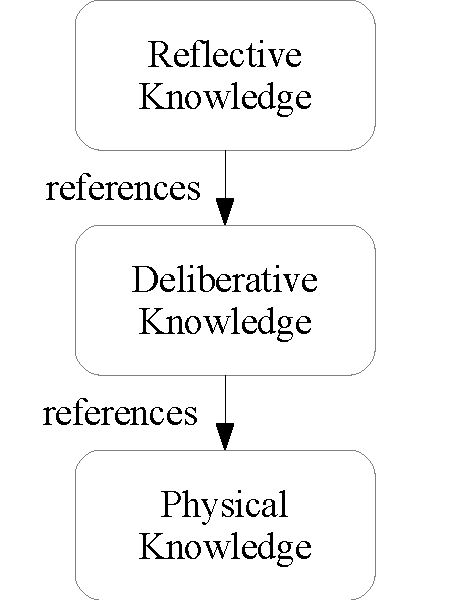
\includegraphics[width=4cm]{gfx/three_knowledge_layers}
  \caption{Three knowledge layers.}
  \label{figure:three_knowledge_layers}
\end{figure}

\section{Natural Language Plans}

SALS includes a simple but powerful planning language that is based on
the interpretation of natural language plans.  Plans are sequences of
commands that can be created, mutated, and executed by a planner in
order to accomplish goals.  The following is an example of a
definition of one of the deliberative plans that the AI in the story
could consider executing:
\begin{samepage}
\begin{Verbatim}
[defplan 'move slowly until over a cube'
  [plan-call [plan 'if a cube is to my left, move slowly
                    left until over a cube, otherwise if a
                    cube is to my right, move slowly right
                    until over a cube']]
  [plan-call [plan 'assert that a cube is below me']]]
\end{Verbatim}
\end{samepage}
This expression defines a new deliberative plan.  The ``defplan''
command is shorthand for ``define plan.''  The first argument to the
defplan expression is the name of the plan: ``move slowly until over a
cube.''  The body of the plan is the remaining sequence of
expressions.  The first expression in the body of this plan is to
interpret and execute the natural language phrase beginning with ``if
a cube...''  The second expression in the body of this plan is to
interpret and execute the natural language phrase beginning with
``assert that...''  This plan positions the AI over a cube and fails
if a cube is not finally below the AI.  If the planner wanted to find
a plan to position the AI over a pyramid, this plan would not help
unless it was slightly modified, replacing all mentions of ``cube''
with ``pyramid.''  In order to help the planner to know what parts of
plans might be analogously replaceable in this way, the SALS planning
language includes optional natural language pattern matching templates
and default frame variable bindings that can be specified for each
plan definition.  The following example shows how this simple plan can
be generalized to allow positioning the AI over a range of shapes:
\begin{samepage}
\begin{Verbatim}
[defplan 'move slowly until over a cube'
  :matches ['move slowly until over a [? shape]']
   :frame [[shape 'cube']]
    [plan-call [plan 'if a [? shape] is to my left, move
                      slowly left until over a [? shape],
                      otherwise if a [? shape] is to my
                      right, move slowly right until over
                      a [? shape]']]
    [plan-call [plan 'assert that a [? shape] is below me']]]
\end{Verbatim}
\end{samepage}
This generalized form of the original plan uses natural language
variables that are specified with a question mark expression, ``?''
Note that there are two optional arguments to the defplan expression
in this example: (1) ``:matches'' and (2) ``:frame.''  The optional
``:matches'' argument specifies a list of potential patterns that this
plan may match as it is being interpreted.  In this case, the variable
expression ``[? shape]'' is allowed to replace the word ``cube'' from
the original name of the plan.  The optional ``:frame'' argument
specifies the default natural language variable bindings.  In this
case, the ``shape'' variable is assigned the natural language phrase
``cube'' by default.  In the body of the generalized form of the plan,
all occurrences of cube have been replaced with the variable
expression ``[? shape]''.  Given this generalized form of the original
plan, the planner can create a new analogous plan as an interpretation
of the natural language phrase ``move slowly until over a pyramid.''
In this way, plans can be communicated to the AI in a natural language
form.  The AI has ``been told'' a total of approximately seventy
simple natural language plans, which can be adapted by analogy to
provide interpretations for a variety of complex possible natural
language plans, including recursive interpretations.  The details of
the planning language will be discussed in
{\mbox{\autoref{chapter:learning_from_being_told_natural_language_plans}}}.

\section{Layers of Learning}

SALS includes an efficient relational learning algorithm in each layer
of planned thinking.  Relational learning in SALS is handled
concurrently with the plan execution in that layer.  In this way, as
plans are executed at full speed, a trace of changes are produced and
sent to a parallel event consuming algorithm that induces abstract
partial states that are used to train a rule learning algorithm.  The
hypotheses that the rule learning algorithm creates are used to
provide explanations as to the parts of the plan that have caused the
traced changes.  I have found that the separation of learning and
planning into concurrent algorithms gives the learning algorithm the
time to work more slowly, while the plan execution can be performed in
bursts at near full speed.

The deliberative layer makes deliberative plans composed of physical
actions in order to accomplish deliberative goals, while the
reflective layer makes reflective plans composed of deliberative
actions in order to accomplish reflective goals.  Deliberative
learning allows the AI to better predict the physical effects of
deliberative plans for physical action, while reflective learning
allows the AI to better predict the deliberative effects of reflective
plans for deliberative action.  The AI is learning at a reflective
level when it thinks to itself, ``I also have new support for the
hypothesis that executing plans that try to accomplish the goal of a
cube being on a pyramid may lead to an expectation failure when
executed.''  This newly supported hypothesis is a reflective
hypothesis about deliberative actions and objects.  The AI
hierarchically assigns credit to the responsible parts of the
executing plan, ``find and execute a recently learned plan to
accomplish my goals,'' that was currently executing at the time of the
unexpected failure.  This precondition for the execution of the plan
is hypothesized to lead to the effects of this action in deliberative
knowledge, ``a deliberative planner is focused on a plan that has
failed.''  The next time that the reflective layer is deciding whether
or not the deliberative planner should execute a given plan, it can
consider this new knowledge and predict whether or not executing the
current plan will put the deliberative planner into a negative or
positive deliberative goal state.  I will discuss the details of SALS'
parallel relational learning algorithm in
{\mbox{\autoref{chapter:learning_asynchronously_from_experience}}}.

\section{Document Overview}

Each of the four contributions of this thesis will be discussed in one
of the following four chapters.  My implementation of the bottom four
layers of an Emotion Machine cognitive architecture is discussed next
in {\mbox{\autoref{chapter:emotion_machine_cognitive_architecture}}}.
In
{\mbox{\autoref{chapter:learning_from_being_told_natural_language_plans}}},
I will describe the natural language planning language that allows
natural language plans to ``be told'' to the AI.  This chapter will
also discuss how the planning process interprets natural language
plans by finding analogies to plans that the AI already knows.  In
{\mbox{\autoref{chapter:learning_asynchronously_from_experience}}}, I
will describe how the AI learns from the experience it gains from
actually executing its plans.  This chapter will describe the
necessary procedurally reflective components that have been used to
attach complex time-intensive learning algorithms to quickly executing
plans of action.  In order to describe my last contribution, I will
describe the SALS virtual machine and reflectively traced programming
language in
{\mbox{\autoref{chapter:virtual_machine_and_programming_language}}}.

{\mbox{\autoref{chapter:related_models}}} relates my AI to other
contemporary cognitive architectures, approaches to reflective
thinking, metacognition, and learning to plan, as well as other
massively multithreaded computer systems.
{\mbox{\autoref{chapter:evaluation}}} evaluates the run-time
performance of the SALS AI and shows a sub-linear increase in
time-complexity for each additional reflective layer.  In
{\mbox{\autoref{chapter:future}}}, I discuss promising directions of
future research for extending this architecture to learn at the top
two layers of the Emotion Machine theory, the self-reflective and
self-conscious layers.  Also, in this chapter I discuss approaches to
overcoming some of the current limitations in the SALS cognitive
architecture.

